\chapter{Análisis}
\label{chap:analisis}

% \section{Interesados}
% \subsection{Usuarios}
% Se han identificado dos tipos de usuarios principales para la aplicación: los gestores de proyectos y los miembros del equipo de proyecto. Ambos tipos de usuarios son agrupados bajo el término genérico de "usuario", ya que ambos interactúan con la aplicación, aunque con diferentes objetivos y necesidades.

% \textbf{Gestores:} Son los usuarios encargados de la dirección y supervisión del proyecto. Tienen visión global del proyecto. A nivel de rol, puede ser un \ac{PM} tradicional, pero también puede ser un rol de liderazgo técnico (Tech Lead, Product Owner, Arquitecto de Software, etc.) que asuma responsabilidades de gestión de proyecto.

% \textbf{Miembros del equipo:} Son los usuarios encargados de la ejecución de las tareas del proyecto. Su interés principal en la aplicación es que el overhead de gestión sea mínimo, y que les permita centrarse en su trabajo. A nivel de rol, pueden ser desarrolladores, diseñadores, analistas, incluso agentes de \ac{IA} que colaboren en el proyecto.

% \subsection{Stakeholders?}

\section{Interesados}
Para asegurar la viabilidad, adopción y éxito comercial de la plataforma, es fundamental identificar a todas las partes interesadas. El ecosistema no solo influye a las personas que interactúan con la interfaz, sino a entidades, organizaciones y servicios cuyo interés o influencia pueden determinar la viabilidad del producto.

A continuación, se establece una diferenciación clara entre el ecosistema general de interesados y los perfiles de usuario que operan directamente el sistema.

\subsection{Matriz de interesados}
En la Tabla \ref{tab:stakeholders} se identifican las principales partes interesadas del producto, evaluando su nivel de influencia sobre el diseño del sistema, su interés principal y la prioridad que se les ha otorgado durante el proceso de análisis de requisitos.

\begin{table}[htbp]
    \centering
    \renewcommand{\arraystretch}{1.4}
    \begin{tabular}{@{} p{3cm} c p{6cm} c @{}}
        \toprule
        \textbf{Interesado} & \textbf{Influencia} & \textbf{Interés Principal} & \textbf{Prioridad} \\
        \midrule
        \textbf{Empresas Cliente (B2B)} & Alta & Aumento de productividad, seguridad y retorno de inversión (ROI). & Alta \\
        
        \textbf{Gestores de Proyectos} & Alta & Visibilidad clara del estado del trabajo, reducción de la carga burocrática y facilidades para la coordinación de equipos. & Alta \\
        
        \textbf{Miembros del Equipo} & Media & Interfaz intuitiva, mínima fricción en el reporte de tareas y claridad en las dependencias sin exceso de microgestión. & Alta \\
        
        \textbf{Proveedores de \ac{IA} y \emph{Cloud}} & Alta & Integración técnica robusta, cumplimiento de los acuerdos de nivel de servicio (SLA) y consumo eficiente de cuotas de API. & Media \\
        
        \textbf{Productos Competidores} & Media & Retención de cuota de mercado, comparación de funcionalidades y estándares de Experiencia de Usuario (UX). & Baja \\
        \bottomrule
    \end{tabular}
    \caption{Matriz de identificación y priorización de partes interesadas.}
    \label{tab:stakeholders}
\end{table}

\subsection{Usuarios del sistema}
Dentro del grupo de interesados con prioridad alta, se extraen los actores que interactúan de forma directa y continua con el \emph{software}. Estos usuarios se agrupan en tres perfiles operativos principales:

\begin{itemize}
    \item \textbf{Gestores y Liderazgo Técnico:} Usuarios encargados de la dirección, planificación y supervisión operativa. Este perfil engloba a \emph{Project Managers}, \emph{Product Owners} y Arquitectos de \emph{Software}. Sus objetivos principales dentro de la herramienta son la configuración de los proyectos, la gestión de roles y accesos, y la detección temprana de cuellos de botella mediante la vista del Árbol de Trabajo.
    
    \item \textbf{Miembros del equipo:} Profesionales encargados de la ejecución técnica o creativa de las tareas (desarrolladores, diseñadores, analistas, etc.). Su interacción con el sistema se basa en el consumo de información (qué hacer y en qué orden) y en la actualización del estado de los elementos de trabajo. Requieren una experiencia libre de fricciones para poder concentrarse en el trabajo de valor.
    
    \item \textbf{Agentes de \ac{IA}:} A diferencia de los sistemas tradicionales, la arquitectura de Leaftask eleva a los agentes de IA a la categoría de actores de primer nivel. Estos entes interactúan con la plataforma de manera análoga a un usuario humano: ejecutan acciones mediante herramientas (\emph{Tools}), leen el progreso de otros usuarios, actualizan estados y se comunican a través de los chats del proyecto.
\end{itemize}

\section{Especificación funcional}
La especificación de los requisitos funcionales se ha realizado con la técnica de historias de usuario, que permite describir las funcionalidades de la aplicación desde la perspectiva del usuario final. Cada historia de usuario se ha formulado siguiendo el formato:
\begin{center}
``Como \textbf{\textit{[tipo de usuario]}}, quiero \textbf{\textit{[funcionalidad]}} para \textbf{\textit{[beneficio]}}.''
\end{center}

Además, cada historia de usuario se ha priorizado utilizando la técnica MoSCoW, que clasifica las funcionalidades en \emph{Must Have} (imprescindibles), \emph{Should Have} (deseables), \emph{Could Have} (interesantes) y \emph{Won't Have} (no necesarias).

También se han organizado las historias de usuario en \emph{épicas}, que agrupan funcionalidades relacionadas entre sí.

\begingroup
\renewcommand{\arraystretch}{1.3}

\begin{longtable}{|p{1.5cm}|p{9cm}|p{3cm}|}
\caption{Historias de usuario}\label{tab:historias}\\

\hline
\textbf{ID} & \textbf{Historia} & \textbf{Prioridad} \\
\hline

\endfirsthead

\multicolumn{3}{|c|}{\textbf{Tabla \thetable{} -- continuación}} \\
\hline
\textbf{ID} & \textbf{Historia} & \textbf{Prioridad} \\
\hline
\endhead

\hline
\multicolumn{3}{|r|}{Continúa en la siguiente página} \\
\hline
\endfoot

\hline
\endlastfoot

\multicolumn{3}{|l|}{\cellcolor{gray!15}\textbf{Épica 1: Identidad y acceso}} \\
\hline

HU-01 &
\textbf{Como} usuario, \textbf{quiero} registrarme mediante OAuth
(Google, Microsoft, Facebook, X)
\textbf{para} acceder a mi espacio de trabajo de forma segura sin gestionar nuevas contraseñas.
& \emph{Must Have} \\
\hline

\multicolumn{3}{|l|}{\cellcolor{gray!15}\textbf{Épica 2: Organización}} \\
\hline

HU-02 &
\textbf{Como} gestor, \textbf{quiero} crear una organización que agrupe proyectos y usuarios
\textbf{para} centralizar la gestión de mi empresa o grupo de trabajo en un solo lugar.
& \emph{Should Have} \\
\hline

HU-03 &
\textbf{Como} gestor, \textbf{quiero} definir roles y permisos de la organización
\textbf{para} permitir a ciertos usuarios diferentes acciones sobre los proyectos de la organización.
& \emph{Should Have} \\
\hline

\multicolumn{3}{|l|}{\cellcolor{gray!15}\textbf{Épica 3: Configuración de proyectos}} \\
\hline

HU-04 &
\textbf{Como} gestor, \textbf{quiero} crear proyectos dentro de una organización o de forma independiente
\textbf{para} organizar el trabajo en diferentes iniciativas o clientes.
& \emph{Must Have} \\
\hline

HU-05 &
\textbf{Como} gestor, \textbf{quiero} poder configurar nombre, abreviación y privacidad de los proyectos
\textbf{para} gestionar el acceso y la visibilidad de la información del proyecto.
& \emph{Must Have} \\
\hline

HU-06 &
\textbf{Como} gestor, \textbf{quiero} definir permisos y roles a nivel de proyecto
\textbf{para} controlar el acceso a la información y funcionalidades del proyecto.
& \emph{Must Have} \\
\hline

HU-07 &
\textbf{Como} gestor, \textbf{quiero} invitar a usuarios a un proyecto
\textbf{para} colaborar con mi equipo en la gestión del proyecto.
& \emph{Must Have} \\
\hline

HU-08 &
\textbf{Como} gestor, \textbf{quiero} clonar un proyecto existente
\textbf{para} reutilizar la estructura y configuración de un proyecto anterior como plantilla en un nuevo proyecto.
& \emph{Could Have} \\
\hline

HU-09 &
\textbf{Como} gestor, \textbf{quiero} añadir campos personalizados a los elementos de trabajo del proyecto
\textbf{para} adaptar la gestión del proyecto a las necesidades específicas de mi equipo o proyecto.
& \emph{Should Have} \\
\hline

\multicolumn{3}{|l|}{\cellcolor{gray!15}\textbf{Épica 4: Elementos de Trabajo}} \\
\hline

HU-10 &
\textbf{Como} usuario, \textbf{quiero} crear y gestionar elementos de trabajo 
\textbf{para} organizar y seguir el progreso de las tareas dentro de un proyecto.
& \emph{Must Have} \\
\hline

HU-11 &
\textbf{Como} usuario, \textbf{quiero} que los elementos de trabajo tengan un set de campos predefinidos (título, descripción, estado, responsable, etiquetas, etc.)
\textbf{para} facilitar la organización y seguimiento de las tareas dentro de un proyecto.
& \emph{Must Have} \\
\hline

HU-12 &
\textbf{Como} usuario, \textbf{quiero} poder dividir el trabajo en elemento de trabajo más pequeños (subtareas)
\textbf{para} gestionar tareas complejas dividiéndolas en partes más manejables
y asignar diferentes responsables a cada parte.
& \emph{Must Have} \\
\hline

HU-13 &
\textbf{Como} miembro del equipo, \textbf{quiero} poder añadir comentarios a los elementos de trabajo y ver un historial de cambios
\textbf{para} facilitar la comunicación y colaboración entre los miembros del equipo, y mantener un registro de las decisiones relacionadas con cada tarea.
& \emph{Should Have} \\
\hline

\multicolumn{3}{|l|}{\cellcolor{gray!15}\textbf{Épica 5: Notificaciones}} \\
\hline

HU-14 &
\textbf{Como} usuario, \textbf{quiero} recibir notificaciones sobre eventos que me afecten (asignación de tareas, cambios en tareas asignadas, menciones, etc.)
\textbf{para} mantenerme informado sobre el progreso del proyecto y las tareas que me afectan.
& \emph{Should Have} \\
\hline

HU-15 &
\textbf{Como} usuario, \textbf{quiero} recibir notificaciones cuando se hace una solicitud de aprobación de una acción que requiera mi aprobación
\textbf{para} poder desbloquear el trabajo de otros miembros del equipo.
& \emph{Should Have} \\
\hline

\multicolumn{3}{|l|}{\cellcolor{gray!15}\textbf{Épica 6: Chats y agentes}} \\
\hline

HU-16 &
\textbf{Como} usuario, \textbf{quiero} poder tener chats, tanto con otros usuarios como con agentes de \ac{IA}
\textbf{para} facilitar la comunicación y colaboración entre los miembros del equipo.
& \emph{Should Have} \\
\hline

HU-17 &
\textbf{Como} usuario, \textbf{quiero} poder crear agentes de \ac{IA} que me ayuden en la gestión del proyecto y tengan un rol específico
\textbf{para} automatizar tareas repetitivas, obtener resúmenes de información relevante, o recibir sugerencias para la gestión del proyecto.
& \emph{Should Have} \\
\hline

HU-18 &
\textbf{Como} gestor, \textbf{quiero} que los agentes de \ac{IA} puedan realizar acciones dentro de la aplicación (crear elementos de trabajo, asignar tareas, enviar notificaciones, etc.)
\textbf{para} automatizar tareas y procesos dentro de la gestión del proyecto.
& \emph{Should Have} \\
\hline

HU-19 &
\textbf{Como} gestor, \textbf{quiero} tener un agente de \ac{IA} predefinido \emph{Daily Standup} \textbf{para} recibir un resumen diario del estado del proyecto, incluyendo tareas pendientes, bloqueos, y progreso general.
& \emph{Could Have} \\
\hline

HU-20 &
\textbf{Como} gestor, \textbf{quiero} tener un agente de \ac{IA} predefinido \emph{Desglose de Trabajo} \textbf{para} poder introducir una tarea compleja y recibir una propuesta de desglose en subtareas más manejables.
& \emph{Could Have} \\
\hline

\multicolumn{3}{|l|}{\cellcolor{gray!15}\textbf{Épica 7: Visualización en Árbol}} \\
\hline

\multicolumn{3}{|p{\dimexpr\linewidth-2\tabcolsep-2\arrayrulewidth\relax}|}{
Tras investigar diferentes opciones para mostrar el estado del proyecto de forma visual, se ha decidido implementar una vista en árbol que permita visualizar la estructura del proyecto y el progreso de cada elemento.
} \\
\hline

HU-21 &
\textbf{Como} usuario, \textbf{quiero} visualizar el proyecto como un grafo donde los elements de trabajo son nodos y las dependencias son conexiones \textbf{para} entender la estructura jerárquica y el orden de ejecución sin entrar al detalle de cada elemento de trabajo.
& \emph{Must Have} \\
\hline

HU-22 &
\textbf{Como} usuario, \textbf{quiero} identificar el tipo de trabajo por la forma del nodo y su esfuerzo estimado por el tamaño \textbf{para} distinguir rápidamente \emph{features} complejas de tareas pequeñas sin leer.
& \emph{Must Have} \\
\hline

HU-23 &
\textbf{Como} usuario, \textbf{quiero} identificar el avance de cada elemento de trabajo por el relleno del nodo \textbf{para} conocer rápidamente el progreso.
& \emph{Must Have} \\
\hline

HU-24 &
\textbf{Como} usuario, \textbf{quiero} ver visualmente cuanto esfuerzo se ha dedicado a un elemento de trabajo respecto a lo planificado \textbf{para} detectar rápidamente desvianciones y poder actuar en consecuencia.
& \emph{Must Have} \\
\hline

HU-25 &
\textbf{Como} usuario, \textbf{quiero} ver en que estado se encuentra un elemento de trabajo mediante su color \textbf{para} coordinarme con el equipo y saber rápidamente si un elemento de trabajo está bloqueado, en progreso, o completado.
& \emph{Must Have} \\
\hline

HU-26 &
\textbf{Como} usuario, \textbf{quiero} ver quién tiene asignado un elemento de trabajo \textbf{para} coordinarme con el equipo.
& \emph{Must Have} \\
\hline

HU-27 &
\textbf{Como} usuario, \textbf{quiero} poder colapsar partes del árbol de trabajo \textbf{para} enfocarme en las partes del proyecto que me interesen sin perder la visión global.
& \emph{Must Have} \\
\hline

\multicolumn{3}{|l|}{\cellcolor{gray!15}\textbf{Épica 8: Perfil}} \\
\hline

HU-28 &
\textbf{Como} usuario, \textbf{quiero} tener un perfil personal indicando mi rol y zona horaria
\textbf{para} que otros usuarios puedan conocer mi rol en los proyectos y para que las notificaciones se ajusten a mi zona horaria.
& \emph{Could Have} \\
\hline

HU-29 &
\textbf{Como} usuario, \textbf{quiero} acumular experiencia en diferentes áreas 
\textbf{para} que gestores y agentes de \ac{IA} puedan recomendarme tareas o proyectos en función de mi experiencia y habilidades.
& \emph{Could Have} \\
\hline

HU-30 &
\textbf{Como} usuario, \textbf{quiero} que mi perfil contenga un indicador de calidad técnica
\textbf{para} que los gestores y agentes de \ac{IA} puedan tener en cuenta no solo mi experiencia, sino también la calidad de mis contribuciones.
& \emph{Could Have} \\
\hline

HU-31 &
\textbf{Como} usuario, \textbf{quiero} que mi perfil contenga  un indicador de la velocidad a la que suelo completar tareas
\textbf{para} que los gestores y agentes de \ac{IA} puedan asignarme tareas teniendo en cuenta no solo mi experiencia y calidad, sino también mi velocidad de trabajo.
& \emph{Could Have} \\
\hline

HU-32 &
\textbf{Como} usuario, \textbf{quiero} que mi perfil contenga un indicador de mi sesgo de optimismo/pesimismo en la estimación de tareas
\textbf{para} que los gestores y agentes de \ac{IA} puedan ajustar las estimaciones de las tareas que me asignen teniendo en cuenta mi sesgo de optimismo/pesimismo.
& \emph{Could Have} \\
\hline

\end{longtable}
\endgroup


\section{Especificación no funcional}
Así mismo, se han identificado los requisitos no funcionales que rigen las restricciones, cualidades y atributos de calidad globales del sistema. Estos requisitos son críticos para garantizar el correcto funcionamiento, la robustez y la viabilidad práctica de la aplicación, abarcando dimensiones esenciales como la seguridad, el rendimiento, la escalabilidad, la disponibilidad, la mantenibilidad y la usabilidad.

\textbf{Seguridad:} 
\begin{itemize}
    \item \textbf{Autenticación estandarizada:} El control de acceso a la plataforma debe gestionarse mediante un sistema de autenticación seguro basado en los estándares industriales OAuth 2.0\cite{rfc6749}.
    \item \textbf{Control de acceso granular:} La protección de los datos e información sensible de las organizaciones y proyectos debe garantizarse mediante un modelo de control de acceso basado en roles (RBAC), aplicando restricciones jerárquicas tanto a nivel global de la organización como a nivel específico de cada proyecto.
    \item \textbf{Gestión de sesiones:} Las sesiones de los usuarios deben expirar automáticamente tras un periodo preconfigurado de inactividad y ofrecer la capacidad de revocar de forma remota e instantánea cualquier sesión activa en caso de compromiso de la cuenta.
\end{itemize}

\textbf{Rendimiento:}
\begin{itemize}
    \item \textbf{Tiempo de respuesta de la API:} El tiempo medio de respuesta del servidor para operaciones síncronas de lectura y escritura de datos debe mantenerse por debajo de los 300~ms para el 95\% de las solicitudes (percentil 95) bajo condiciones normales de carga.
    \item \textbf{Procesamiento asíncrono de IA:} Las tareas con alta carga computacional, tales como la generación de resúmenes por parte de agentes de \ac{IA} o el desglose automatizado de elementos de trabajo complejos, deben procesarse de manera asíncrona, notificando al usuario el inicio del proceso.
    \item \textbf{Fluidez de la interfaz (Vista en árbol):} El motor de renderizado en el cliente debe asegurar una tasa de refresco fluida y cercana a los 60 \ac{FPS} durante la interacción visual y la manipulación del grafo de tareas, minimizando el impacto del re-renderizado en proyectos complejos.
\end{itemize}

\textbf{Escalabilidad:}
\begin{itemize}
    \item \textbf{Escalado horizontal:} La arquitectura del sistema debe permitir el escalado horizontal independiente de sus componentes (servicios de aplicación, pasarelas de agentes de \ac{IA} y bases de datos), facilitando el aislamiento de cargas de trabajo intensivas sin degradar el núcleo de la aplicación.
    \item \textbf{Concurrencia del sistema:} El sistema debe ser capaz de manejar de forma eficiente hasta 1000 usuarios concurrentes activos y soportar picos de carga de hasta 100 operaciones por segundo sin experimentar una degradación perceptible en los tiempos de respuesta.
\end{itemize}

\textbf{Disponibilidad:}
\begin{itemize}
    \item \textbf{Tiempo de actividad (Uptime):} La aplicación debe garantizar una disponibilidad continua del 99.9\% del tiempo, excluyendo exclusivamente las ventanas de tiempo previamente notificadas para tareas de mantenimiento programado.
    \item \textbf{Tolerancia a fallos:} El sistema debe implementar mecanismos de recuperación automática y aislamiento de fallos, tales como políticas de reintentos, para mitigar caídas de servicios externos o de las APIs de proveedores de \ac{IA}.
\end{itemize}

\textbf{Mantenibilidad:}
\begin{itemize}
    \item \textbf{Arquitectura desacoplada:} El diseño del código fuente debe seguir un patrón arquitectónico modular, desacoplado y de alta cohesión (como la arquitectura hexagonal o limpia\cite{martin2017clean}), separando estrictamente la lógica del dominio de los detalles de infraestructura para facilitar su comprensión, mantenimiento y extensión.
    \item \textbf{Cobertura de pruebas:} Las capas de la aplicación que albergan las reglas de negocio y los casos de uso centrales deben contar con una cobertura de pruebas unitarias automatizadas de al menos un 80\%.
    \item \textbf{Inyección de configuración:} Todos los parámetros operativos, variables de entorno, credenciales de servicios externos e hiperparámetros de los modelos de \ac{IA} deben estar completamente externalizados del código fuente, permitiendo modificaciones en caliente sin necesidad de recompilar o redesplegar la aplicación.
    \item \textbf{Análisis estático obligatorio:} El flujo de integración continua (\ac{CI}) debe requerir la superación obligatoria de un análisis estático de código para garantizar los estándares de calidad del software, el control de la complejidad ciclomática y la ausencia de deuda técnica crítica antes de cada despliegue.
\end{itemize}

\textbf{Usabilidad:}
\begin{itemize}
    \item \textbf{Heurísticas de diseño:} La interfaz de usuario deberá cumplir con los criterios de usabilidad validados mediante una evaluación heurística basada en los 10 principios de Nielsen y Molich~\cite{nielsen1990heuristic}.
    \item \textbf{Accesibilidad web:} La aplicación debe observar las directrices esenciales de accesibilidad web, asegurando relaciones de contraste cromático adecuadas en los nodos del árbol de tareas y el soporte para la navegación y operación mediante teclado en los formularios principales~\cite{w3c2018wcag21}.
\end{itemize}

\section{Modelado del Dominio}
El análisis del núcleo de Leaftask se ha abordado desde la perspectiva del \ac{DDD} \cite{evans2004ddd}, priorizando la comprensión de las reglas de negocio. Dado que la gestión de proyectos asistida por inteligencia artificial presenta una alta complejidad conceptual, el dominio principal se ha descompuesto en múltiples \emph{Bounded Contexts} \cite{fowler2014boundedcontext}.

En esta fase de análisis, cada \emph{Bounded Context} establece un límite estricto donde un subconjunto del modelo de dominio tiene total validez y autonomía. Esta separación permite aislar y entender áreas de responsabilidad claras (como la gestión de identidades, la estructura de los elementos de trabajo o la coordinación de agentes automatizados), garantizando que el modelo refleje fielmente la realidad del negocio antes de tomar decisiones.

A continuación, se detallan los pilares de este análisis, comenzando por el vocabulario compartido que vertebra el sistema, hasta llegar a la representación de los datos de cada contexto.

\subsection{Lenguaje ubicuo}

Siguiendo los principios del \ac{DDD}, se ha definido un lenguaje ubicuo que unifica la terminología utilizada por los desarrolladores y los usuarios, facilitando la comunicación y el entendimiento mutuo entre ambos grupos. Este lenguaje se ha construido a partir de los términos y conceptos más relevantes para la gestión de proyectos, y se ha utilizado de forma consistente en toda la documentación, los diagramas y el código fuente de la aplicación.

\begin{description}
    \item[Organización:] Entidad principal que agrupa a múltiples usuarios y proyectos bajo un mismo espacio de trabajo, centralizando la gestión de permisos y roles a nivel corporativo o de grupo.
    \item[Proyecto:] Iniciativa de trabajo acotada que contiene un conjunto estructurado de elementos de trabajo orientados a un objetivo común.
    \item[Miembro del Equipo:] Entidad asignada a un proyecto para colaborar en su ejecución. Un miembro del equipo puede ser tanto un usuario humano (desarrollador, diseñador) como un Agente de \ac{IA}.
    \item[Gestor:] Rol encargado de la configuración, supervisión y administración de proyectos y organizaciones.
    \item[Agente de \ac{IA}:] Miembro del equipo automatizado que colabora en el proyecto. Actúa bajo un rol específico y tiene capacidad para interactuar con el sistema de manera análoga a un usuario humano.
    \item[Elemento de Trabajo (\emph{Work Item}):] Unidad básica de gestión dentro de un proyecto. Representa una tarea, funcionalidad o incidencia, y encapsula información como estado, responsable, esfuerzo estimado y dependencias.
    \item[Árbol de Trabajo:] Representación visual, jerárquica e interactiva del conjunto de elementos de trabajo de un proyecto en forma de grafo.
    \item[Nodo:] Representación gráfica de un único Elemento de Trabajo dentro del Árbol de Trabajo. Sus atributos visuales (forma, tamaño, color y relleno) comunican instantáneamente el tipo de trabajo, el esfuerzo estimado, el estado y el avance.
    \item[Estado:] Situación operativa actual de un elemento de trabajo en su ciclo de vida (pendiente, en progreso, bloqueado, completado).
    \item[Rol:] Conjunto de responsabilidades y nivel de autoridad asignado a un Miembro del Equipo  dentro de una Organización o Proyecto. Define qué acciones puede realizar en el sistema.
    \item[Permiso:] Autorización explícita y granular para ejecutar una acción específica o acceder a un recurso concreto (ej. crear proyecto, invitar usuario, modificar elemento de trabajo). Los permisos se agrupan conformando un Rol.
    \item[Campo Personalizado:] Atributo dinámico definido para extender la información predefinida de los Elementos de Trabajo, adaptándolos a las necesidades específicas de un proyecto.
    \item[Aprobación:] Petición formal generada dentro del ciclo de vida de una acción que requiere la validación explícita de un usuario con los permisos adecuados para desbloquear el progreso.
\end{description}

\subsection{Modelo de Dominio}
Tras definir el lenguaje ubicuo, es necesario establecer cómo interactúan estos conceptos entre sí. El modelo conceptual se centra exclusivamente en las reglas de negocio y las relaciones estructurales de las entidades principales de Leaftask.

En la Figura \ref{fig:uml-dominio} se muestra el diagrama de clases \ac{UML}. Para facilitar su comprensión, el dominio se ha modelado utilizando interfaces polimórficas que resuelven relaciones complejas, agrupándose en los siguientes bloques funcionales:

\begin{figure}[htbp]
    \centering
    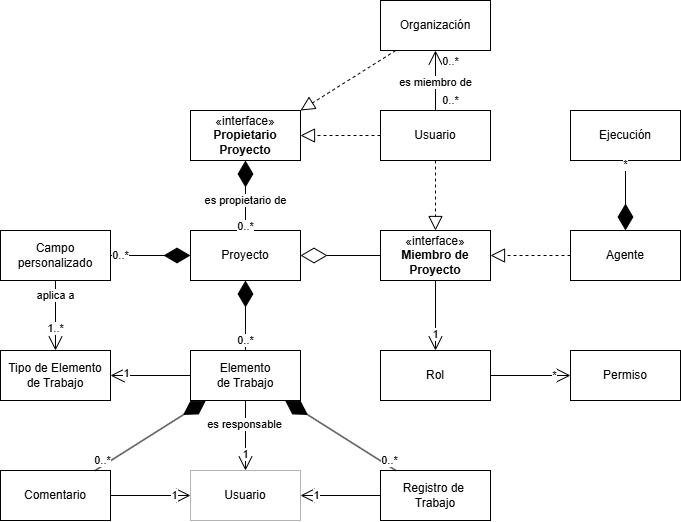
\includegraphics[width=1\textwidth]{images/content/Analisis/uml-dominio.png}
    \caption{Diagrama UML del modelo conceptual de dominio de las entidades principales.}
    \label{fig:uml-dominio}
\end{figure}

\subsubsection{Organizaciones}
El sistema resuelve la pertenencia de los proyectos de forma flexible mediante la interfaz \textbf{Propietario Proyecto}:
\begin{itemize}
    \item Un \textbf{Proyecto} debe pertenecer exactamente a un propietario.
    \item Este propietario puede ser una \textbf{Organización} (agrupando a múltiples usuarios que son miembros de la misma) o un \textbf{Usuario} individual (para proyectos de carácter personal).
    \item A su vez, un Usuario puede ser miembro de múltiples Organizaciones, estableciendo una relación de muchos a muchos (\emph{0..*}).
\end{itemize}

\subsubsection{Miembros de Proyectos}
La colaboración dentro de los proyectos abstrae la naturaleza del participante mediante la interfaz \textbf{Miembro de Proyecto}:
\begin{itemize}
    \item Un Proyecto está compuesto por múltiples miembros. Esta interfaz es implementada tanto por \textbf{Usuarios} (humanos) como por \textbf{Agentes} (Inteligencia Artificial), otorgándoles a ambos la capacidad de interactuar con el sistema.
    \item Todo miembro dentro de un proyecto tiene asignado exactamente un \textbf{Rol}.
    \item Cada Rol se compone de un conjunto granular de \textbf{Permisos} (\emph{0..*}), definiendo de forma estricta qué acciones puede llevar a cabo el miembro en ese contexto específico.
\end{itemize}

\subsubsection{Elementos de Trabajo y Campos Personalizados}
El núcleo de gestión pivota sobre la entidad \textbf{Elemento de Trabajo}, que se adapta dinámicamente a las necesidades del proyecto:
\begin{itemize}
    \item Un Proyecto contiene múltiples Elementos de Trabajo. Cada uno de ellos debe estar catalogado bajo un \textbf{Tipo de Elemento de Trabajo} (por ejemplo: \emph{Bug}, Tarea, Épica).
    \item Para dotar al sistema de flexibilidad, un Proyecto puede definir múltiples \textbf{Campos Personalizados}.
    \item Estos campos no se aplican globalmente, sino que se asocian explícitamente a uno o varios Tipos de Elemento de Trabajo (\emph{1..*}), garantizando que cada elemento solo solicite la información pertinente a su naturaleza.
\end{itemize}

\subsubsection{Interacción, Trazabilidad y Automatización}
El dominio garantiza el seguimiento completo de la actividad y la ejecución asíncrona:
\begin{itemize}
    \item Un Elemento de Trabajo tiene asignado exactamente un Usuario responsable de su resolución.
    \item Los Usuarios pueden generar \textbf{Comentarios} y \textbf{Registros de Trabajo} (\emph{Work Logs}). Ambas entidades mantienen una doble relación de composición: pertenecen simultáneamente al Elemento de Trabajo donde se generaron y al Usuario que las emitió.
    \item Por último, los Agentes de IA encapsulan su actividad en instancias de \textbf{Ejecución}. Un Agente puede tener múltiples ejecuciones a lo largo de su ciclo de vida, lo que permite trazar el histórico de sus acciones y decisiones de forma independiente.
\end{itemize}